\documentclass[a4paper,12pt]{ctexart}

\usepackage{geometry}

\geometry{a4paper, left=2.5cm, right=2.5cm, top=2.5cm, bottom=2.5cm}

\usepackage{amsmath}

\usepackage{caption}

\usepackage{graphicx}

\usepackage{listings}

\usepackage{xcolor}

\usepackage{fontspec}

\usepackage{url}

\setmainfont{Microsoft YaHei}

\setkeys{Gin}{width=\textwidth, keepaspectratio}

\lstset{
	basicstyle=\footnotesize\ttfamily,
	frame=single,
	numbers=none,
	backgroundcolor=\color{gray!5},
	breaklines=true,
	breakatwhitespace=false,
	columns=flexible,
	xleftmargin=4pt,
	xrightmargin=4pt,
	breakindent=1em
}

\begin{document}
	
	\title{系统开发工具基础 第四周实验报告}
	\author{涂睿昕---25020007115}
	\maketitle
	
	\section{实验概述}
	本次实验为系统开发工具基础第四周课上实验，实验环境为VirtualBox中的Ubuntu虚拟机。本次完成四项课上实验：建立可执行的本地质量门禁、Make构建系统实验、API与jq生成Markdown报告、综合交付测试实验。实验主要练习代码质量工具ruff与pytest、Make构建系统、curl+jq文本处理、Python包综合交付测试；掌握本地质量门禁编写、Make依赖与伪目标、JSON命令行解析、缺陷复现修复、wheel打包哈希校验的完整工程流程。
	
	\section{课上实验题目}
	
	\subsection{q13：建立可执行的本地质量门禁}
	\subsubsection{题目要求}
	复用q10完成的greetlab包，在q13中建立轻量本地质量检查。在pyproject.toml添加ruff与pytest最小配置；补充正常姓名、空白姓名两组测试用例；运行ruff format、ruff check、pytest修复全部告警；编写check.sh脚本依次执行格式检查、静态检查、单元测试，脚本执行返回码为0代表全部门禁通过。
	
	\subsubsection{实现过程与关键命令}
	\begin{lstlisting}[language=bash]
		cd ~/sdt-course/week4
		cp -r ../week3/q10 q13
		cd q13
		python3 -m venv q13-venv
		source q13-venv/bin/activate
		pip install ruff pytest build
		pip install -e .
		ruff format .
		chmod +x check.sh
		./check.sh
		deactivate
		rm -rf q13-venv build dist __pycache__ .pytest_cache src/*.egg-info
	\end{lstlisting}
	
	check.sh脚本内容：
	\begin{lstlisting}[language=bash]
		#!/usr/bin/env bash
		set -e
		
		echo "=== ruff format check ==="
		ruff format --check
		
		echo "=== ruff lint check ==="
		ruff check
		
		echo "=== pytest run ==="
		pytest
	\end{lstlisting}
	
	pyproject.toml补充ruff、pytest配置，保留原有包构建配置。
	
	\subsubsection{运行结果}
	执行\texttt{./check.sh}，ruff格式检查、静态代码检查全部通过；pytest两组测试用例全部PASS；脚本退出码为0，本地质量门禁全部校验成功。
	\begin{lstlisting}
		=== ruff format check ===
		6 files already formatted
		=== ruff lint check ===
		All checks passed!
		=== pytest run ===
		=============================================== test session starts ===============================================
		platform linux -- Python 3.12.3, pytest-9.1.1, pluggy-1.6.0
		rootdir: /home/lin/sdt-course/week4/q13
		configfile: pyproject.toml
		testpaths: .
		collected 2 items                                                                                                 
		
		test_greet.py ..                                                                                            [100%]
		
		================================================ 2 passed in 0.03s ================================================
	\end{lstlisting}
	
	\begin{figure}[htbp]
		\centering
		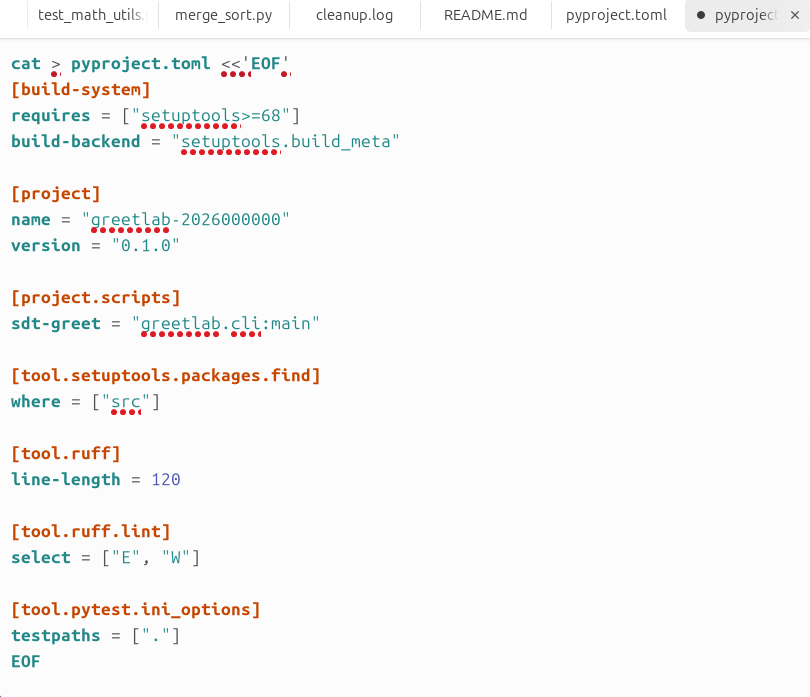
\includegraphics[width=0.9\textwidth]{q13p1.png}
		\caption{q13pyproject.toml修改后截图}
		\label{fig:q13_1}
	\end{figure}
	
	\begin{figure}[htbp]
		\centering
		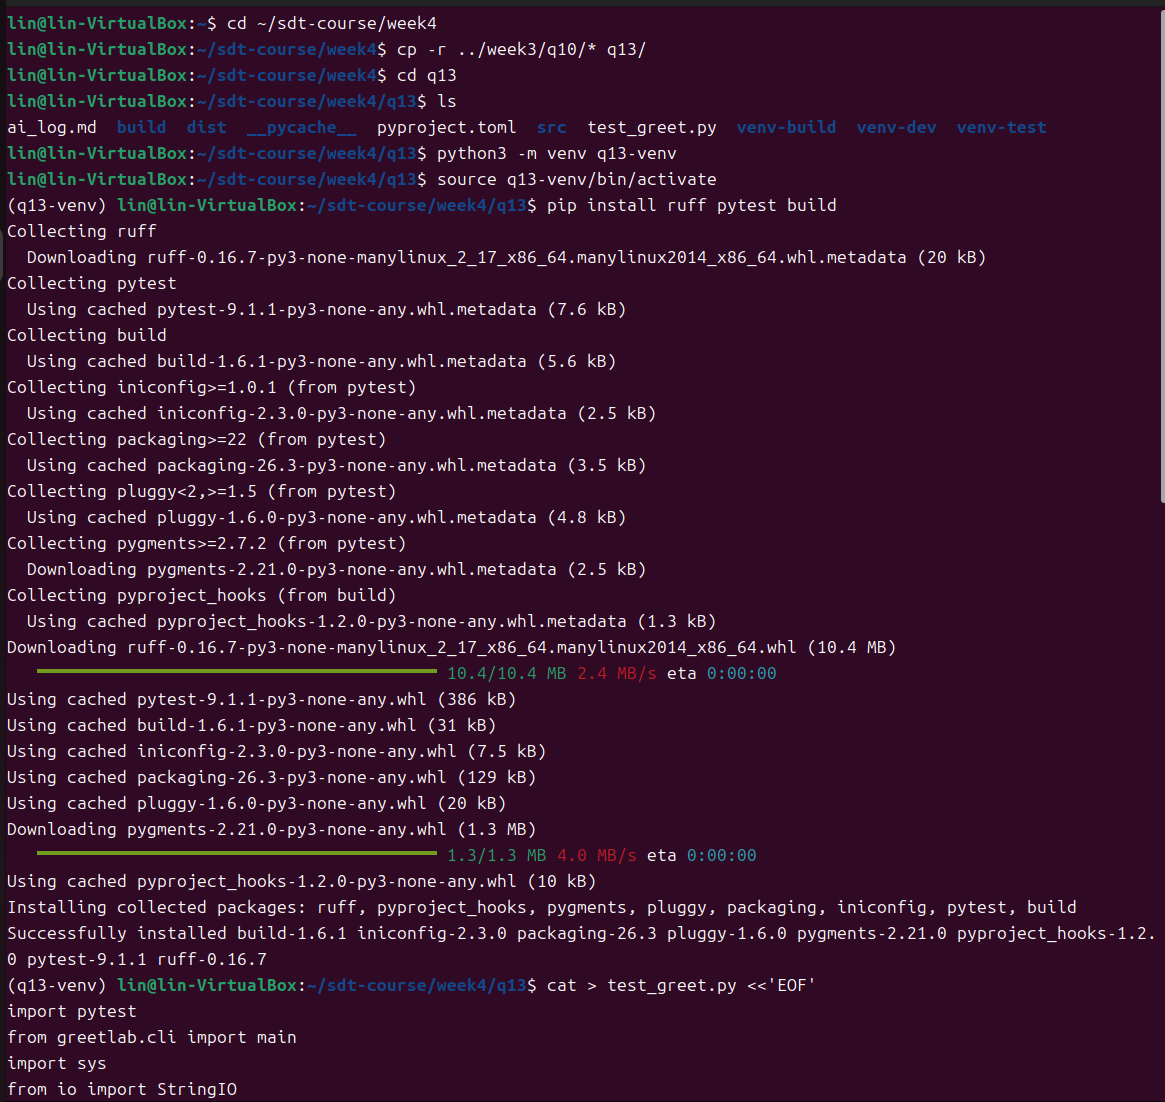
\includegraphics[width=0.9\textwidth]{q13p2.png}
		\caption{q13运行截图1}
		\label{fig:q13_2}
	\end{figure}
	
	\begin{figure}[htbp]
		\centering
		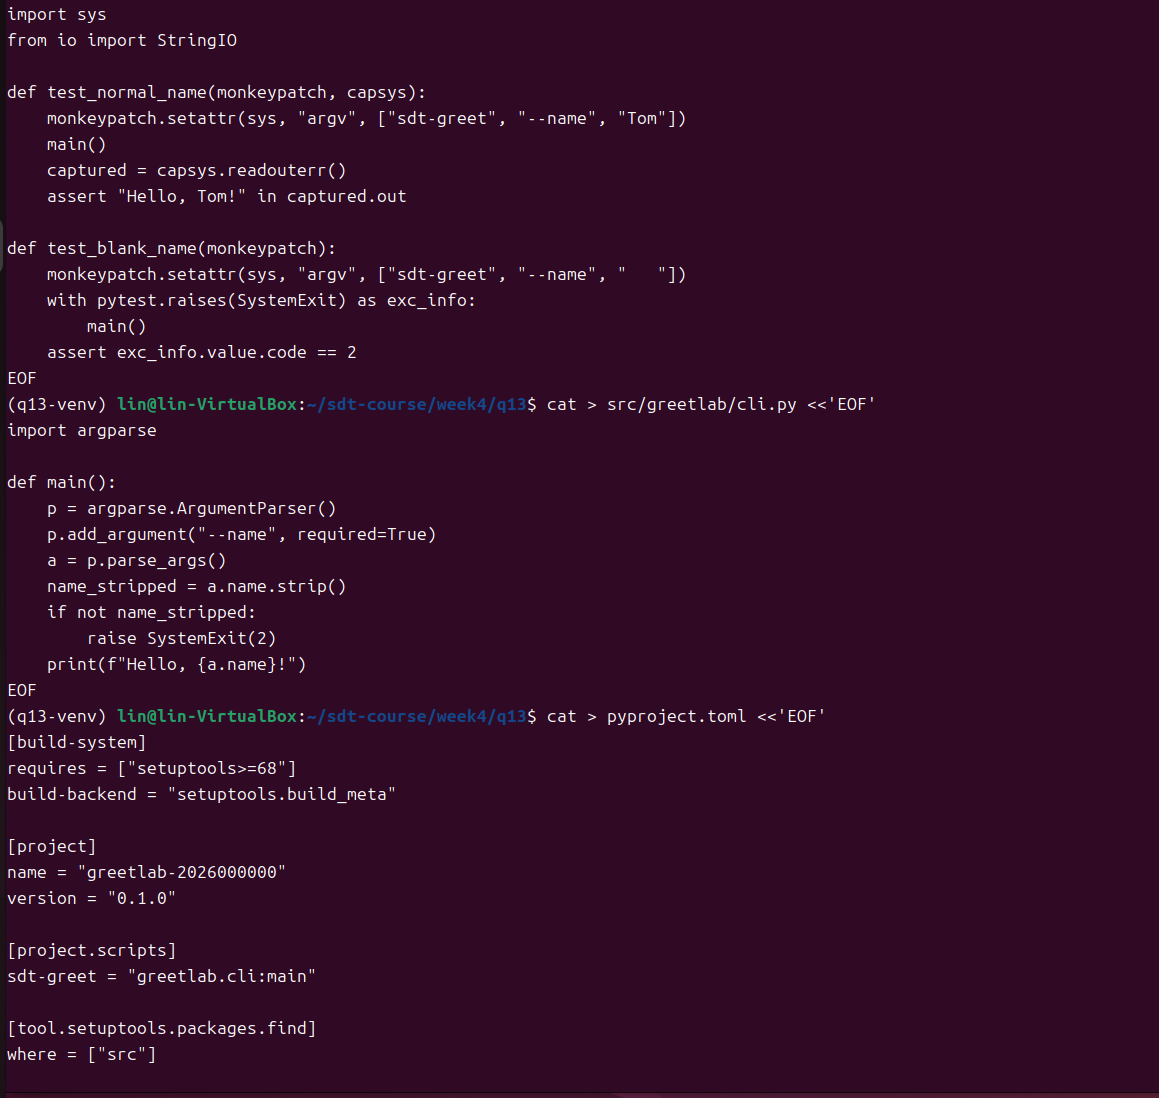
\includegraphics[width=0.9\textwidth]{q13p3.png}
		\caption{q13运行截图2}
		\label{fig:q13_3}
	\end{figure}
	
	\begin{figure}[htbp]
		\centering
		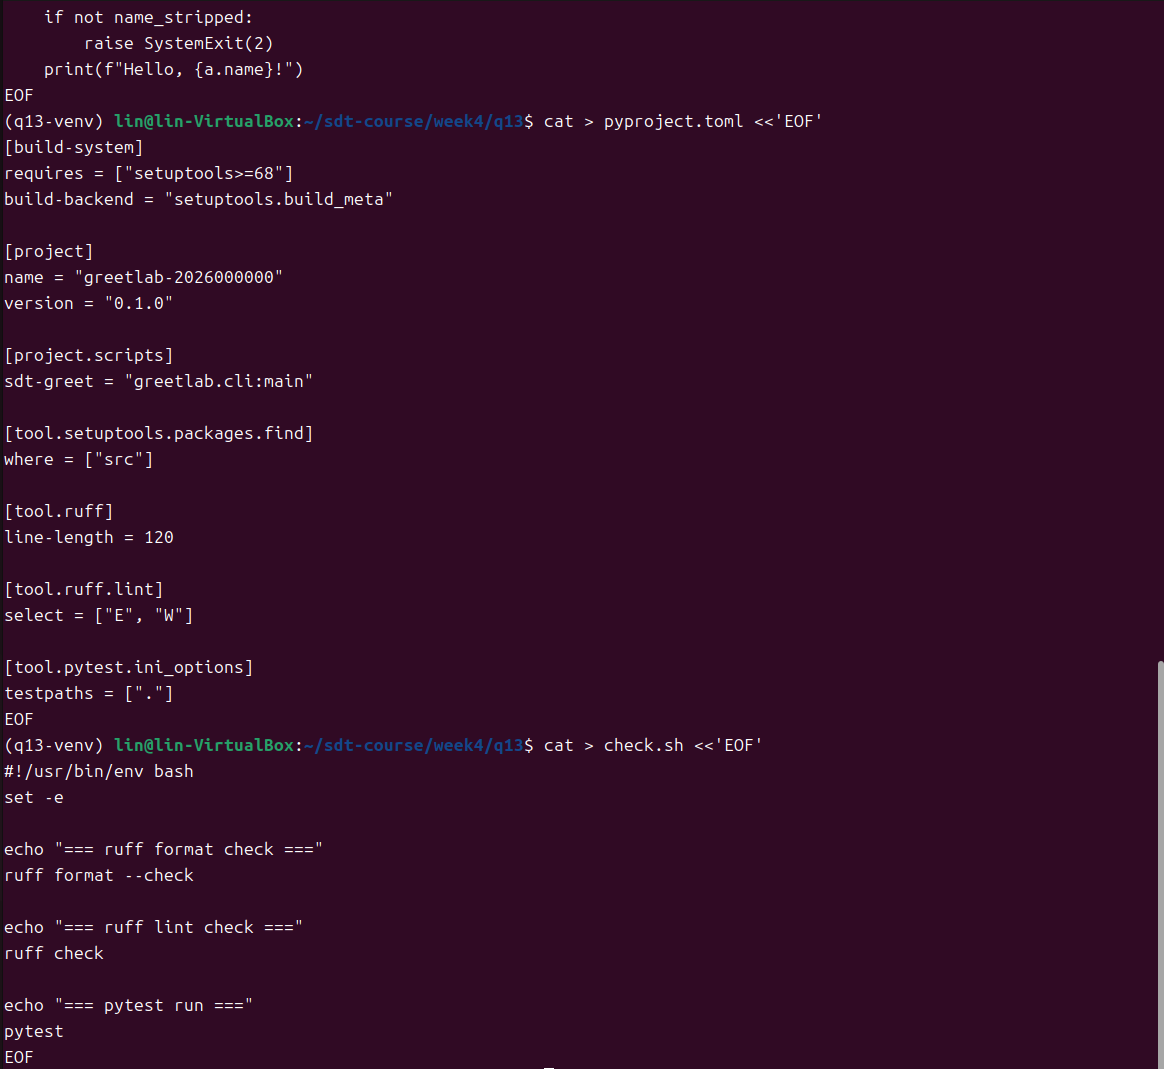
\includegraphics[width=0.9\textwidth]{q13p4.png}
		\caption{q13运行截图3}
		\label{fig:q13_4}
	\end{figure}
	
	\begin{figure}[htbp]
		\centering
		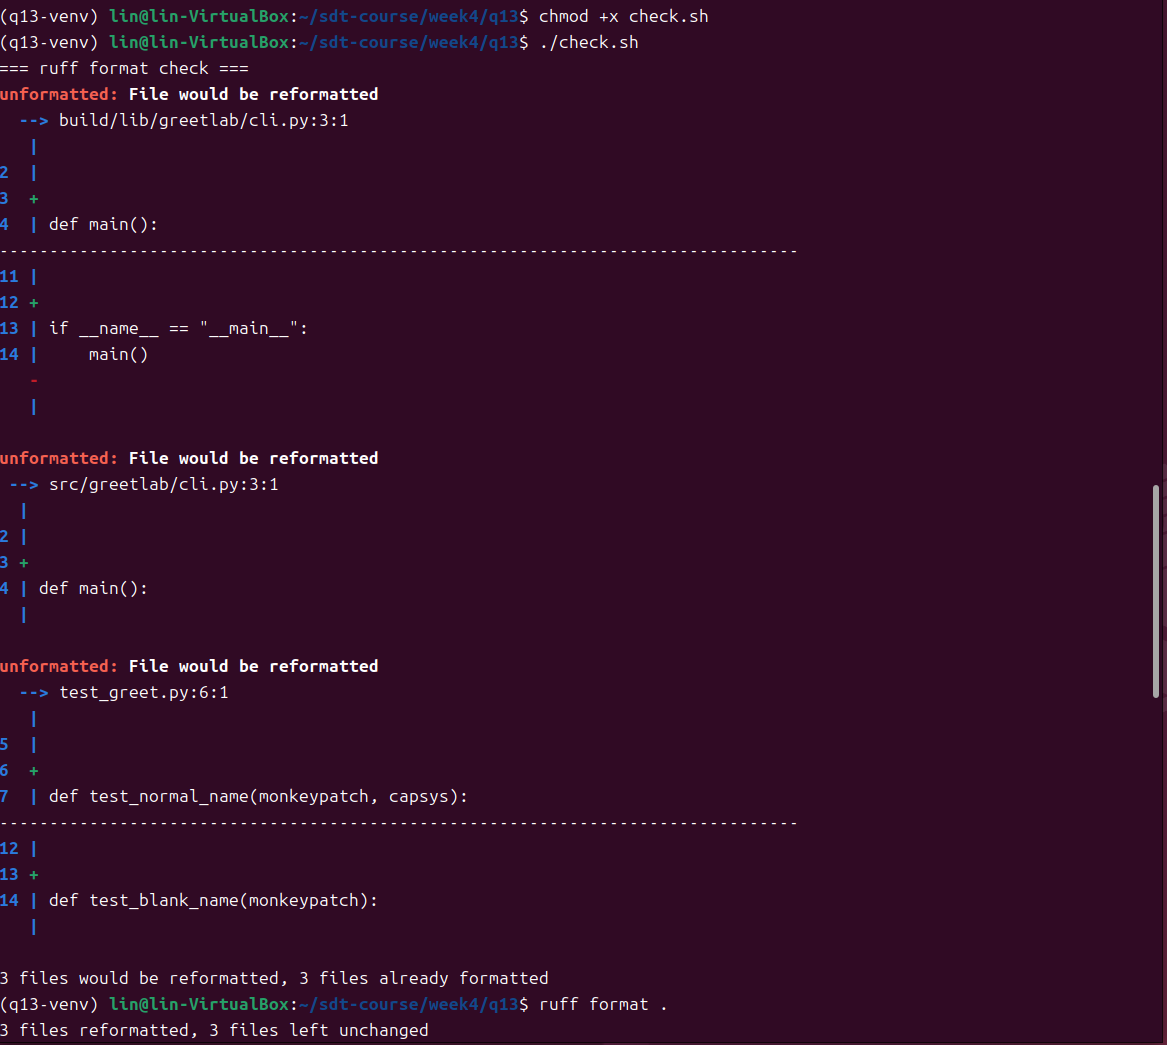
\includegraphics[width=0.9\textwidth]{q13p5.png}
		\caption{q13运行截图4}
		\label{fig:q13_5}
	\end{figure}
	
	\begin{figure}[htbp]
		\centering
		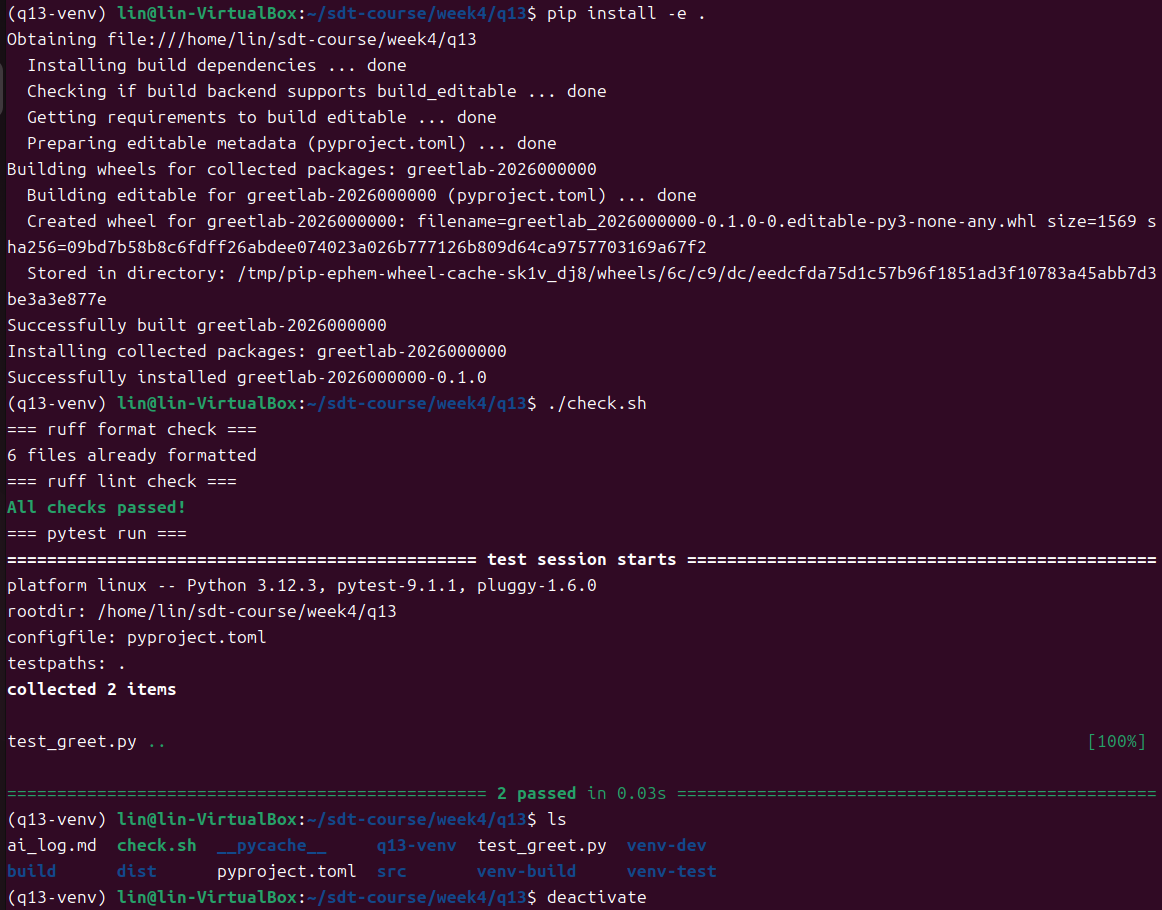
\includegraphics[width=0.9\textwidth]{q13p6.png}
		\caption{q13运行截图5}
		\label{fig:q13_6}
	\end{figure}
	
	\subsubsection{遇到的问题与解决}
	\begin{itemize}
		\item 问题1：执行\texttt{ruff format --check}时报错\texttt{File would be reformatted}，文件格式不符合规范，门禁脚本直接失败。
		
		解决：运行\texttt{ruff format .}对源码执行自动格式化，修复换行空行格式问题，之后再执行格式检查；删除自动生成的build临时目录，避免工具扫描构建产物。
		
		\item 问题2：pytest收集测试用例时报\texttt{ModuleNotFoundError: No module named 'greetlab'}，无法导入src下的包模块。
		
		解决：在虚拟环境中执行可编辑模式安装\texttt{pip install -e .}，将本地源码包注册到虚拟环境，Python可正常导入greetlab模块。
		
		\item 问题3：多次测试后遗留多个虚拟环境\texttt{venv‑build}、\texttt{venv‑dev}、\texttt{venv‑test}，以及egg‑info、build缓存目录，文件数量庞大，不应当提交版本库。
		
		解决：实验结束后使用\texttt{rm -rf}整体删除整套虚拟环境目录，同步清理build、dist、*.egg‑info、Python字节码缓存，只保留作业源码与脚本。
	\end{itemize}
	
	\subsection{q14：让Make只重建真正受影响的产物}
	\subsubsection{题目要求}
	创建data.csv、stats.py、build\_report.py、report.md源文件；编写Makefile，实现all、stats.txt、report.txt、clean规则；准确书写全部依赖；将all、clean声明为伪目标.PHONY；验证首次构建、无修改不重新执行、数据源变更触发重构建、clean仅删除生成产物。
	
	\subsubsection{实现过程与关键命令}
	\begin{lstlisting}[language=bash]
		cd ~/sdt-course/week4/q14
		cat > data.csv <<'EOF'
		name,value
		alpha,2
		beta,3
		gamma,5
		EOF
		
		cat > stats.py <<'EOF'
		import csv
		
		with open("data.csv") as f:
		total = sum(int(r["value"]) for r in csv.DictReader(f))
		
		with open("stats.txt", "w") as f:
		f.write(str(total))
		EOF
		
		cat > build_report.py <<'EOF'
		text = open("report.md").read()
		total = open("stats.txt").read()
		open("report.txt", "w").write(f"{text}\nTotal: {total}\n")
		EOF
		
		cat > report.md <<'EOF'
		# Data Report
		EOF
		
		cat > Makefile <<'EOF'
		.PHONY: all clean
		
		all: stats.txt report.txt
		
		stats.txt: data.csv stats.py
		python3 stats.py
		
		report.txt: stats.txt build_report.py report.md
		python3 build_report.py
		
		clean:
		rm -f stats.txt report.txt
		EOF
		
		make all
		make all
		touch data.csv
		make all
		make clean
	\end{lstlisting}
	
	Makefile完整内容：
	\begin{lstlisting}[language=make]
		.PHONY: all clean
		
		all: stats.txt report.txt
		
		stats.txt: data.csv stats.py
		python3 stats.py
		
		report.txt: stats.txt build_report.py report.md
		python3 build_report.py
		
		clean:
		rm -f stats.txt report.txt
	\end{lstlisting}
	
	\subsubsection{运行结果}
	第一次\texttt{make all}生成stats.txt与report.txt；无修改再次make提示nothing to be done；touch data.csv触发重新构建两个产物；make clean仅删除生成文件，原始源码全部保留。
	\begin{lstlisting}
		python3 stats.py
		python3 build_report.py
		
		make: 对“all”无需做任何事。
		
		python3 stats.py
		python3 build_report.py
		
		rm -f stats.txt report.txt
	\end{lstlisting}
	
	\begin{figure}[htbp]
		\centering
		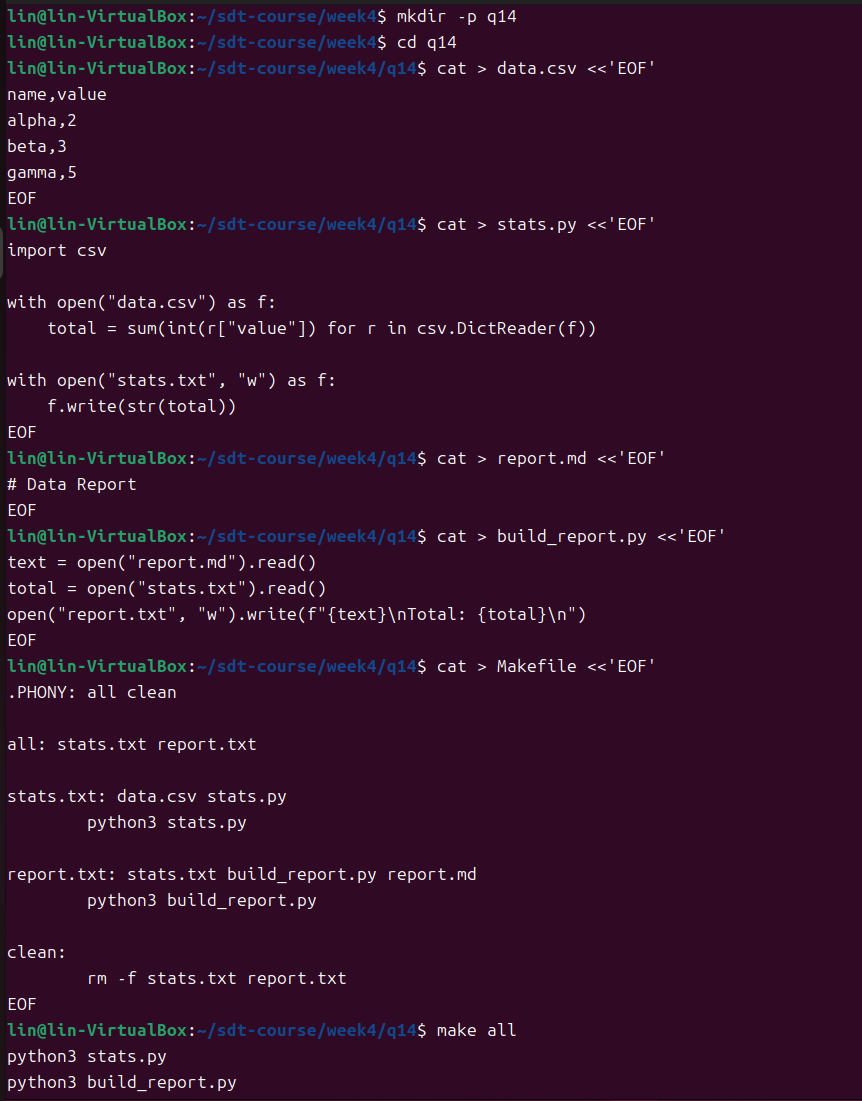
\includegraphics[width=0.9\textwidth]{q14p1.png}
		\caption{q14运行截图1}
		\label{fig:q14_1}
	\end{figure}
	
	\begin{figure}[htbp]
		\centering
		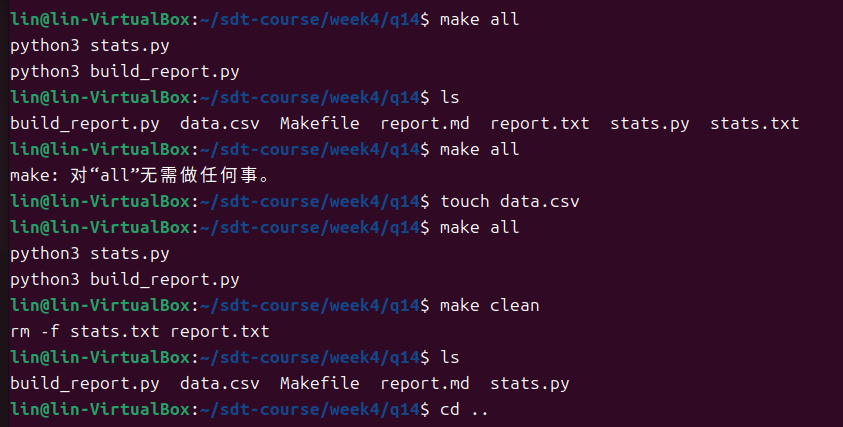
\includegraphics[width=0.9\textwidth]{q14p2.png}
		\caption{q14运行截图2}
		\label{fig:q14_2}
	\end{figure}
	
	\subsubsection{遇到的问题与解决}
	\begin{itemize}
		\item 问题1：编写Makefile时忘记声明\texttt{.PHONY: all clean}，若目录下恰好存在名为all或clean的文件，make将不会执行对应规则。
		
		解决：将伪目标all与clean写进\texttt{.PHONY}声明，告诉make它们不是磁盘上的真实文件，总是执行对应配方。
		
		\item 问题2：依赖关系书写不全，如report.txt只写依赖stats.txt，遗漏build\_report.py、report.md；修改脚本或md文件不会触发重新构建。
		
		解决：完整列出所有影响输出的源文件作为依赖，只要任意依赖发生变更就会重新执行构建命令。
		
	\end{itemize}
	
	\subsection{q15：把本地API数据转换为可读报告}
	\subsubsection{题目要求}
	创建packages.json；启动本地python http.server 8000服务；编写api\_report.sh脚本，使用curl获取接口JSON，jq筛选status为active且downloads不少于100，按downloads降序、name升序；输出summary.md，包含标题与name/version/downloads三列Markdown表格。
	
	\subsubsection{实现过程与关键命令}
	\begin{lstlisting}[language=bash]
		cd ~/sdt-course/week4/q15
		cat > packages.json <<'EOF'
		[
		{"name":"alpha","status":"active","downloads":120,"version":"1.2.0"},
		{"name":"beta","status":"inactive","downloads":900,"version":"2.0.0"},
		{"name":"gamma","status":"active","downloads":450,"version":"1.5.1"},
		{"name":"delta","status":"active","downloads":450,"version":"0.9.0"},
		{"name":"epsilon","status":"active","downloads":80,"version":"3.1.0"}
		]
		EOF
		
		cat > api_report.sh <<'EOF'
		#!/usr/bin/env bash
		set -e
		
		curl -fsS http://127.0.0.1:8000/packages.json > raw.json
		
		jq -r '
		map(select(.status=="active" and .downloads >= 100))
		| sort_by(-.downloads, .name)
		| "name|version|downloads",
		"---|---|---",
		(.[] | "\(.name)|\(.version)|\(.downloads)")
		' raw.json > table.tmp
		
		cat > summary.md <<MD
		# Active Packages Report
		
		$(cat table.tmp)
		MD
		
		rm -f raw.json table.tmp
		EOF
		
		chmod +x api_report.sh
		# 新开终端执行 python3 -m http.server 8000
		./api_report.sh
		cat summary.md
		# http服务终端Ctrl‑C关闭服务
	\end{lstlisting}
	
	api\_report.sh脚本：
	\begin{lstlisting}[language=bash]
			#!/usr/bin/env bash
		set -e
		
		curl -fsS http://127.0.0.1:8000/packages.json > raw.json
		
		jq -r '
		map(select(.status=="active" and .downloads >= 100))
		| sort_by(-.downloads, .name)
		| "name|version|downloads",
		"---|---|---",
		(.[] | "\(.name)|\(.version)|\(.downloads)")
		' raw.json > table.tmp
		
		cat > summary.md <<MD
		# Active Packages Report
		
		$(cat table.tmp)
		MD
		
		rm -f raw.json table.tmp
	\end{lstlisting}
	
	\subsubsection{运行结果}
	脚本调用curl拿到JSON数据，经过jq过滤排序，输出summary.md，生成格式正确的Markdown三列表格；过滤掉inactive与downloads小于100的条目；downloads相同时按照name字典序升序。
	\begin{lstlisting}
		# Active Packages Report
		
		name|version|downloads
		---|---|---
		delta|0.9.0|450
		gamma|1.5.1|450
		alpha|1.2.0|120
	\end{lstlisting}
	
	\begin{figure}[htbp]
		\centering
		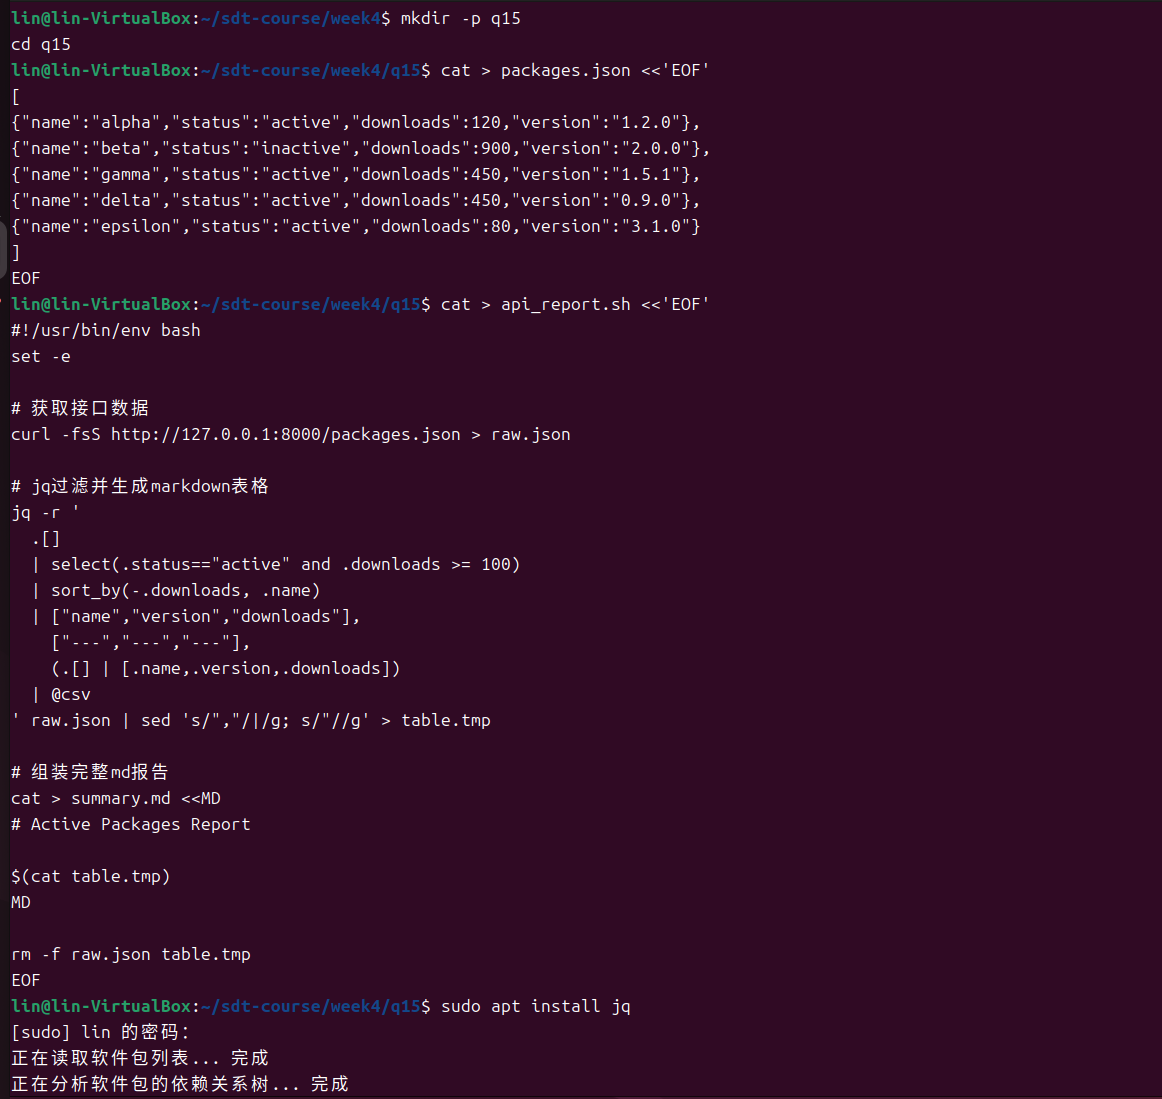
\includegraphics[width=0.9\textwidth]{q15p1.png}
		\caption{q15运行截图1}
		\label{fig:q15_1}
	\end{figure}
	
	\begin{figure}[htbp]
		\centering
		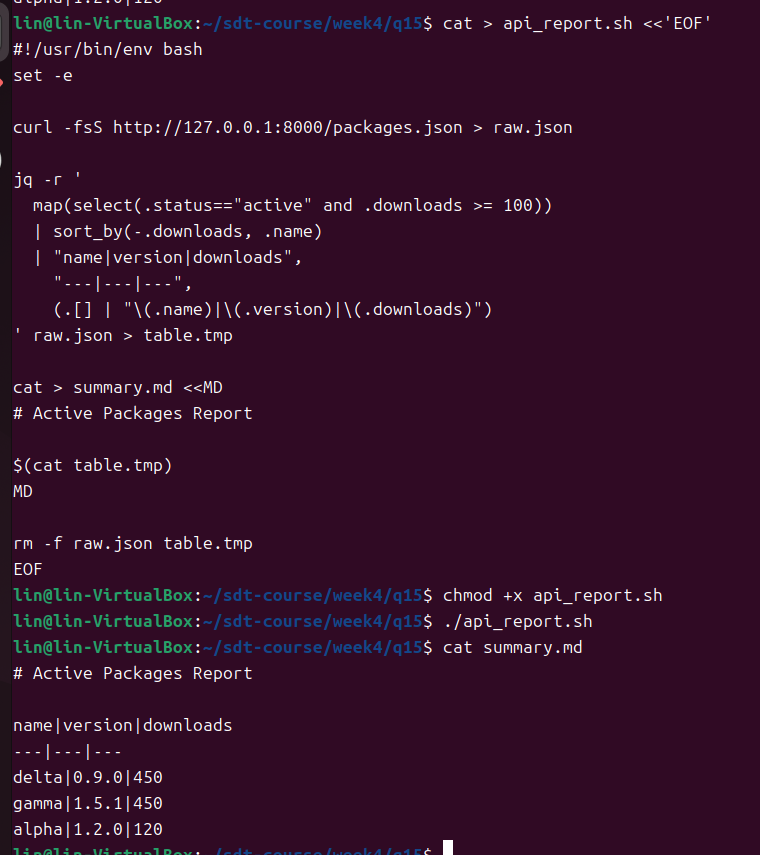
\includegraphics[width=0.9\textwidth]{q15p2.png}
		\caption{q15运行截图2}
		\label{fig:q15_2}
	\end{figure}
	
	\begin{figure}[htbp]
		\centering
		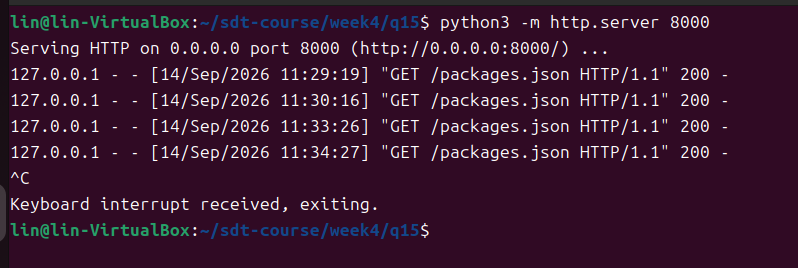
\includegraphics[width=0.9\textwidth]{q15p3.png}
		\caption{q15http服务终端截图}
		\label{fig:q15_3}
	\end{figure}
	
	\subsubsection{遇到的问题与解决}
	\begin{itemize}
		
		\item 问题1：排序逻辑颠倒，未实现下载量降序、同名次按名称升序；直接输出原始JSON数组没有做markdown表格格式转换。
		
		解决：使用\texttt{sort\_by(-.downloads, .name)}完成复合排序；通过\texttt{@csv}输出后用sed替换分隔符转为Markdown表格语法。
		
		\item 问题2：jq中对数组使用\texttt{.[]}展开之后再调用\texttt{sort\_by}，得到单个JSON对象，报Cannot index string with string "downloads"。
		
		解决：使用\texttt{map(select(...))}在数组容器内完成过滤，保证传给\texttt{sort\_by}的仍然是数组对象，排序完成后再展开输出表格行。
		
		\item 问题3：通过\texttt{@csv}输出后使用sed替换分隔符，替换不完全，出现逗号与竖线混合，Markdown表格列分隔错乱。
		
		解决：放弃csv中转，直接在jq内部使用\texttt{join("|")}，输出原生以竖线分隔的表格行，避免sed文本替换带来的格式错误。
		
		\item 问题4：使用数组+join("|")的方式，只会在数组首尾添加竖线，数组内部字段之间保留逗号，表格列分隔符错乱。
		解决：改用jq字符串插值\verb!"\(.name)|\(.version)|\(.downloads)"!，逐行直接拼接完整Markdown表格行，保证三列之间都是竖线分隔。
		
		\item 问题5：jq中将表头写成数组形式，-r原始输出模式打印完整JSON数组，产生多余方括号与引号，破坏报告格式。
		
		解决：表头与表格分隔行直接定义为字符串字面量，仅循环生成数据行，保证全部输出为纯文本表格。
		
		\item 问题6：脚本产生raw.json、table.tmp临时中间文件残留。
		
		解决：脚本末尾增加rm清理临时文件，只保留最终产物summary.md。
		
	\end{itemize}
	
	\subsection{q16：修复并交付一个陌生的小型工具仓库}
	\subsubsection{题目要求}
	复制q13项目作为q16；故意篡改代码制造bug，运行check.sh确认测试失败；修复业务代码，门禁全部通过；编写Makefile包含check、build、clean；check调用./check.sh，build执行python3 -m build生成wheel包；clean删除build、dist；运行make check、make build，计算wheel文件sha256哈希；完成一次干净git提交。
	
	\subsubsection{实现过程与关键命令}
	\begin{lstlisting}[language=bash]
		cd ~/sdt-course/week4
		cp -r q13 q16
		cd q16
		python3 -m venv q16-venv
		source q16-venv/bin/activate
		pip install ruff pytest build
		pip install -e .
		
		# 故意制造bug
		cat > src/greetlab/cli.py <<'EOF'
		import argparse
		
		def main():
		p = argparse.ArgumentParser()
		p.add_argument("--name", required=True)
		a = p.parse_args()
		# 故意bug：写死输出字面量
		print("Hello, name!")
		EOF
		
		ruff format .
		./check.sh
		
		# 修复bug
		cat > src/greetlab/cli.py <<'EOF'
		import argparse
		
		def main():
		p = argparse.ArgumentParser()
		p.add_argument("--name", required=True)
		a = p.parse_args()
		name_stripped = a.name.strip()
		if not name_stripped:
		raise SystemExit(2)
		print(f"Hello, {a.name}!")
		EOF
		
		ruff format .
		./check.sh
		
		cat > Makefile <<'EOF'
		.PHONY: check build clean
		
		check:
		./check.sh
		
		build:
		python3 -m build
		
		clean:
		rm -rf build dist
		EOF
		
		make check
		make build
		sha256sum dist/*.whl
		deactivate
		rm -rf q16-venv build dist __pycache__ .pytest_cache src/*.egg-info
	\end{lstlisting}
	
	q16的Makefile：
	\begin{lstlisting}[language=make]
		.PHONY: check build clean
		
		check:
		./check.sh
		
		build:
		python3 -m build
		
		clean:
		rm -rf build dist
	\end{lstlisting}
	
	\subsubsection{运行结果}
	篡改cli.py硬编码输出字面量，门禁中ruff格式通过，pytest测试用例断言失败；修复代码后check.sh全部绿灯；make check执行质量门禁；make build在dist目录生成wheel源码分发包；sha256sum得到wheel文件完整性哈希摘要。
	\begin{lstlisting}
		=== ruff format check ===
		4 files already formatted
		=== ruff lint check ===
		All checks passed!
		=== pytest run ===
		================================================= test session starts =================================================
		platform linux -- Python 3.12.3, pytest-9.1.1, pluggy-1.6.0
		rootdir: /home/lin/sdt-course/week4/q16
		configfile: pyproject.toml
		testpaths: .
		collected 2 items                                                                                                     
		
		test_greet.py FF                                                                                                [100%]
		
		====================================================== FAILURES =======================================================
		__________________________________________________ test_normal_name ___________________________________________________
		
		monkeypatch = <_pytest.monkeypatch.MonkeyPatch object at 0x740914f18620>
		capsys = <_pytest.capture.CaptureFixture object at 0x740914f18740>
		
		def test_normal_name(monkeypatch, capsys):
		monkeypatch.setattr(sys, "argv", ["sdt-greet", "--name", "Tom"])
		main()
		captured = capsys.readouterr()
		>       assert "Hello, Tom!" in captured.out
		E       AssertionError: assert 'Hello, Tom!' in 'Hello, name!\n'
		E        +  where 'Hello, name!\n' = CaptureResult(out='Hello, name!\n', err='').out
		
		test_greet.py:11: AssertionError
		___________________________________________________ test_blank_name ___________________________________________________
		
		monkeypatch = <_pytest.monkeypatch.MonkeyPatch object at 0x740914f18ef0>
		
		def test_blank_name(monkeypatch):
		monkeypatch.setattr(sys, "argv", ["sdt-greet", "--name", "   "])
		>       with pytest.raises(SystemExit) as exc_info:
		E       Failed: DID NOT RAISE SystemExit
		
		test_greet.py:16: Failed
		------------------------------------------------ Captured stdout call -------------------------------------------------
		Hello, name!
		=============================================== short test summary info ===============================================
		FAILED test_greet.py::test_normal_name - AssertionError: assert 'Hello, Tom!' in 'Hello, name!\n'
		FAILED test_greet.py::test_blank_name - Failed: DID NOT RAISE SystemExit
		================================================== 2 failed in 0.03s ==================================================
		
		=== ruff format check ===
		4 files already formatted
		=== ruff lint check ===
		All checks passed!
		=== pytest run ===
		================================================= test session starts =================================================
		platform linux -- Python 3.12.3, pytest-9.1.1, pluggy-1.6.0
		rootdir: /home/lin/sdt-course/week4/q16
		configfile: pyproject.toml
		testpaths: .
		collected 2 items                                                                                                     
		
		test_greet.py ..                                                                                                [100%]
		
		================================================== 2 passed in 0.01s ==================================================
		
		./check.sh
		=== ruff format check ===
		4 files already formatted
		=== ruff lint check ===
		All checks passed!
		=== pytest run ===
		================================================= test session starts =================================================
		platform linux -- Python 3.12.3, pytest-9.1.1, pluggy-1.6.0
		rootdir: /home/lin/sdt-course/week4/q16
		configfile: pyproject.toml
		testpaths: .
		collected 2 items                                                                                                     
		
		test_greet.py ..                                                                                                [100%]
		
		================================================== 2 passed in 0.01s ==================================================
		
		Successfully built greetlab_2026000000-0.1.0.tar.gz and greetlab_2026000000-0.1.0-py3-none-any.whl
		
		2c33f7032736c3d85dc322b59461b21545983e9d70d37f694e3e844c4b916b73  dist/greetlab_2026000000-0.1.0-py3-none-any.whl
	\end{lstlisting}
	
	\begin{figure}[htbp]
		\centering
		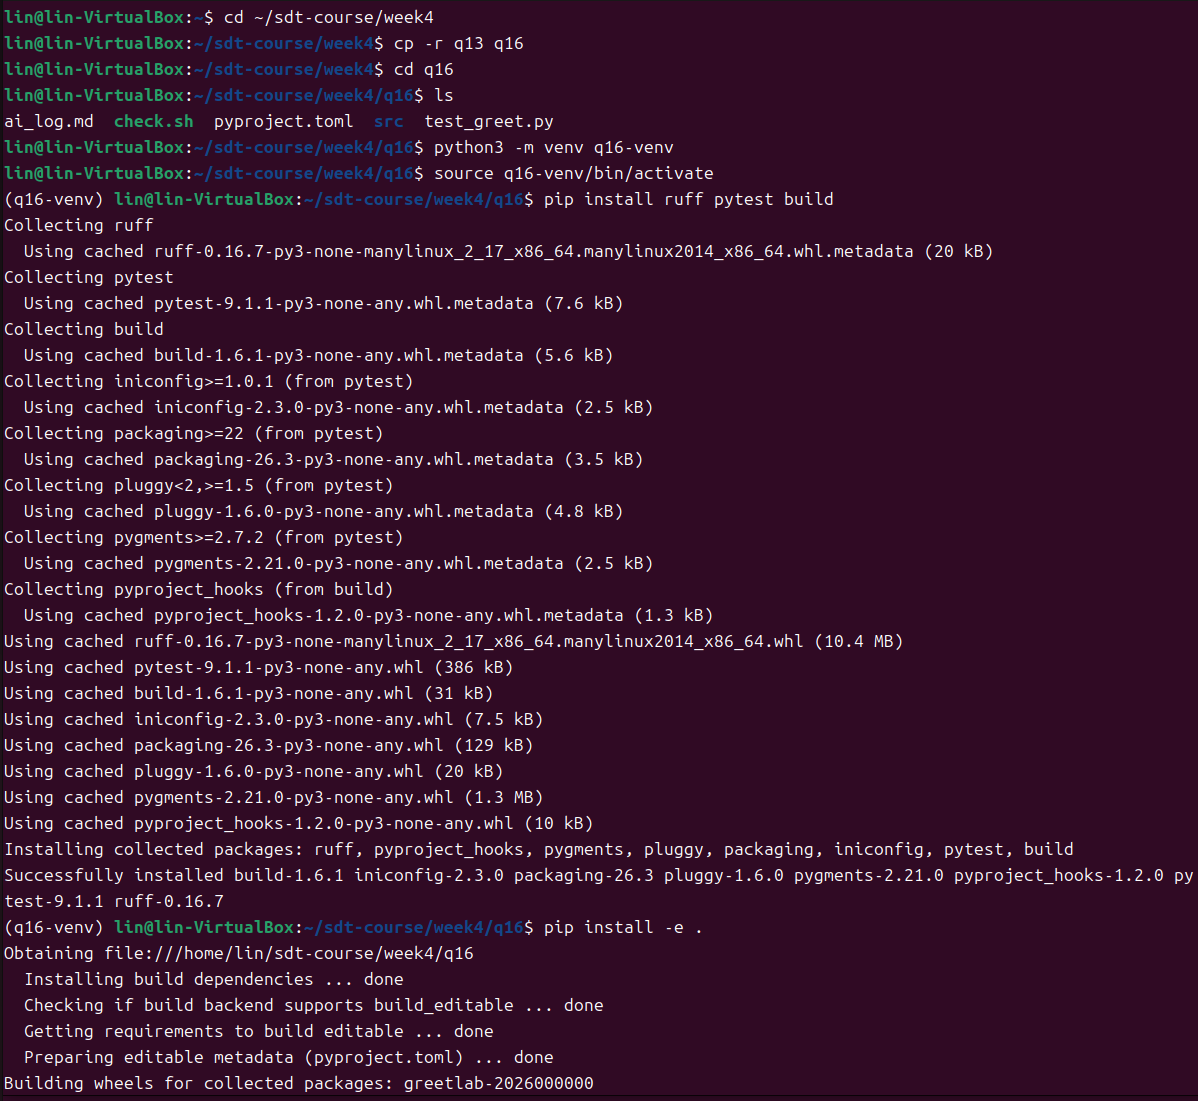
\includegraphics[width=0.9\textwidth]{q16p1.png}
		\caption{q16运行截图1}
		\label{fig:q16_1}
	\end{figure}
	
	\begin{figure}[htbp]
		\centering
		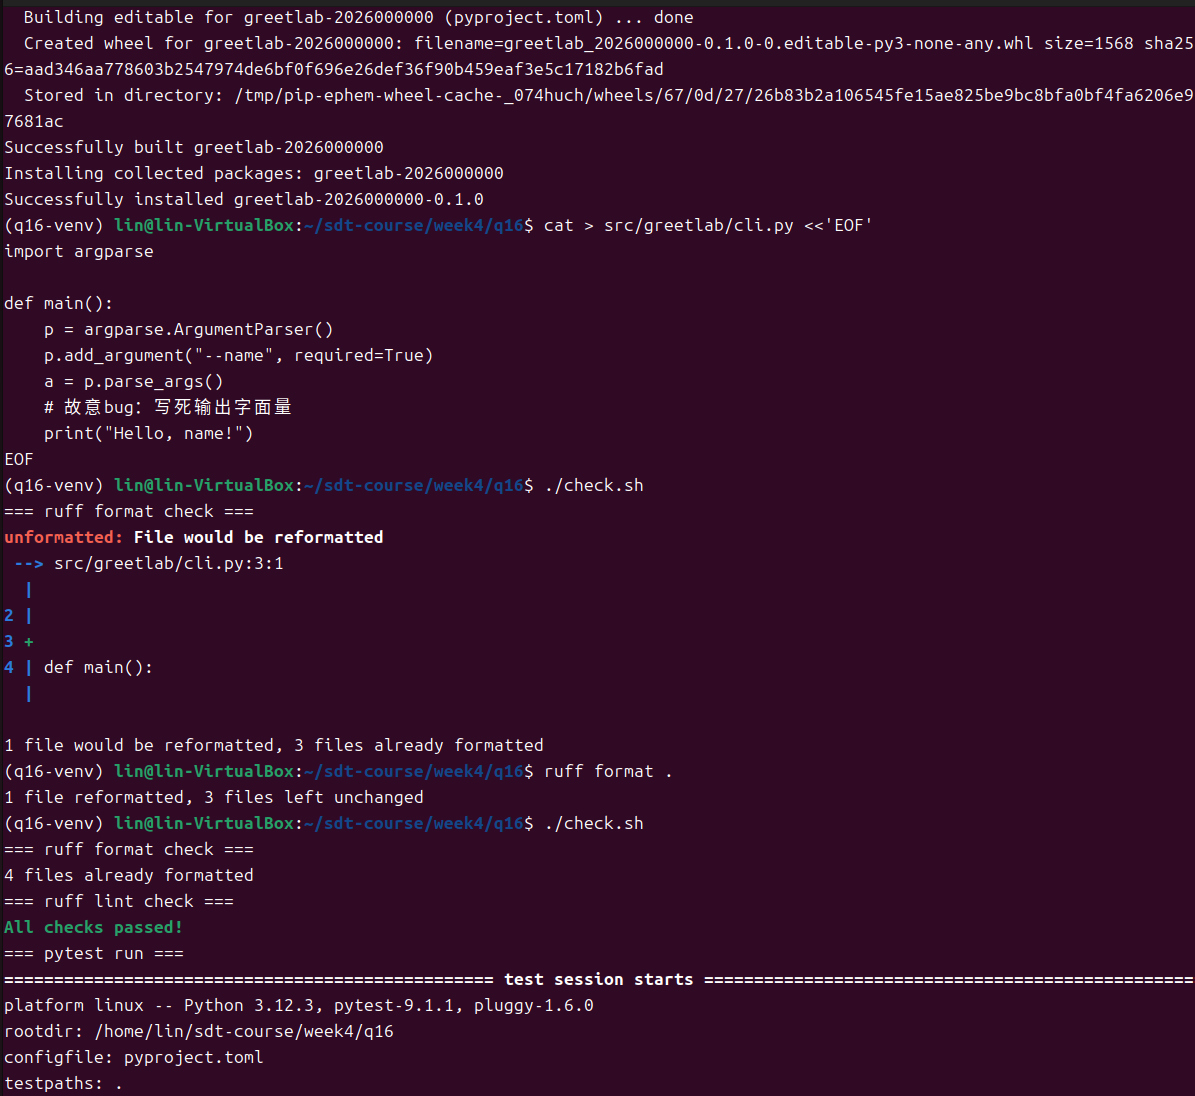
\includegraphics[width=0.9\textwidth]{q16p2.png}
		\caption{q16运行截图2}
		\label{fig:q16_2}
	\end{figure}
	
	\begin{figure}[htbp]
		\centering
		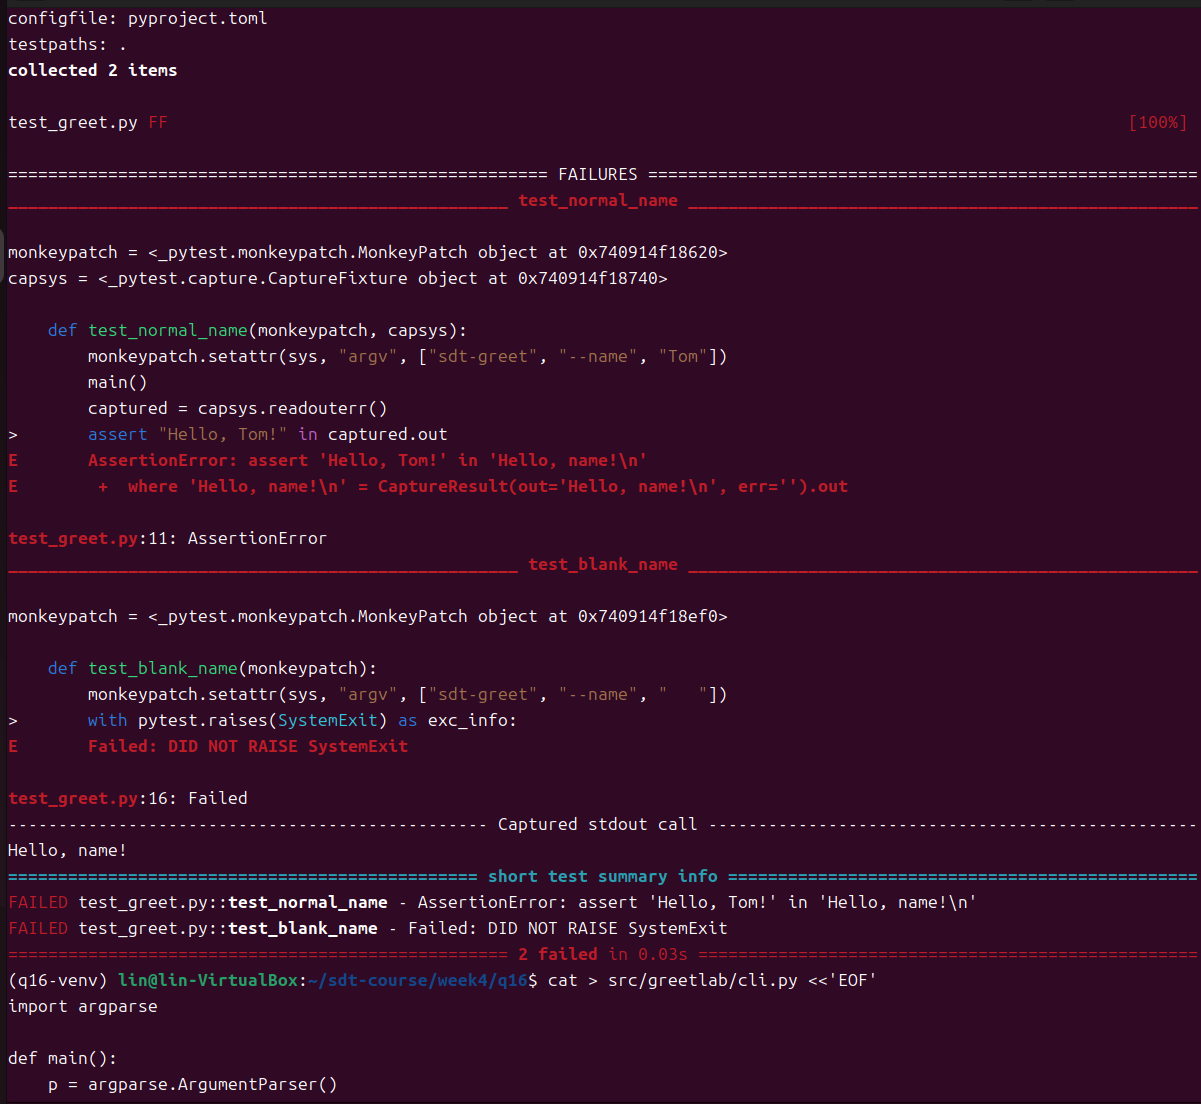
\includegraphics[width=0.9\textwidth]{q16p3.png}
		\caption{q16运行截图3}
		\label{fig:q16_3}
	\end{figure}
	
	\begin{figure}[htbp]
		\centering
		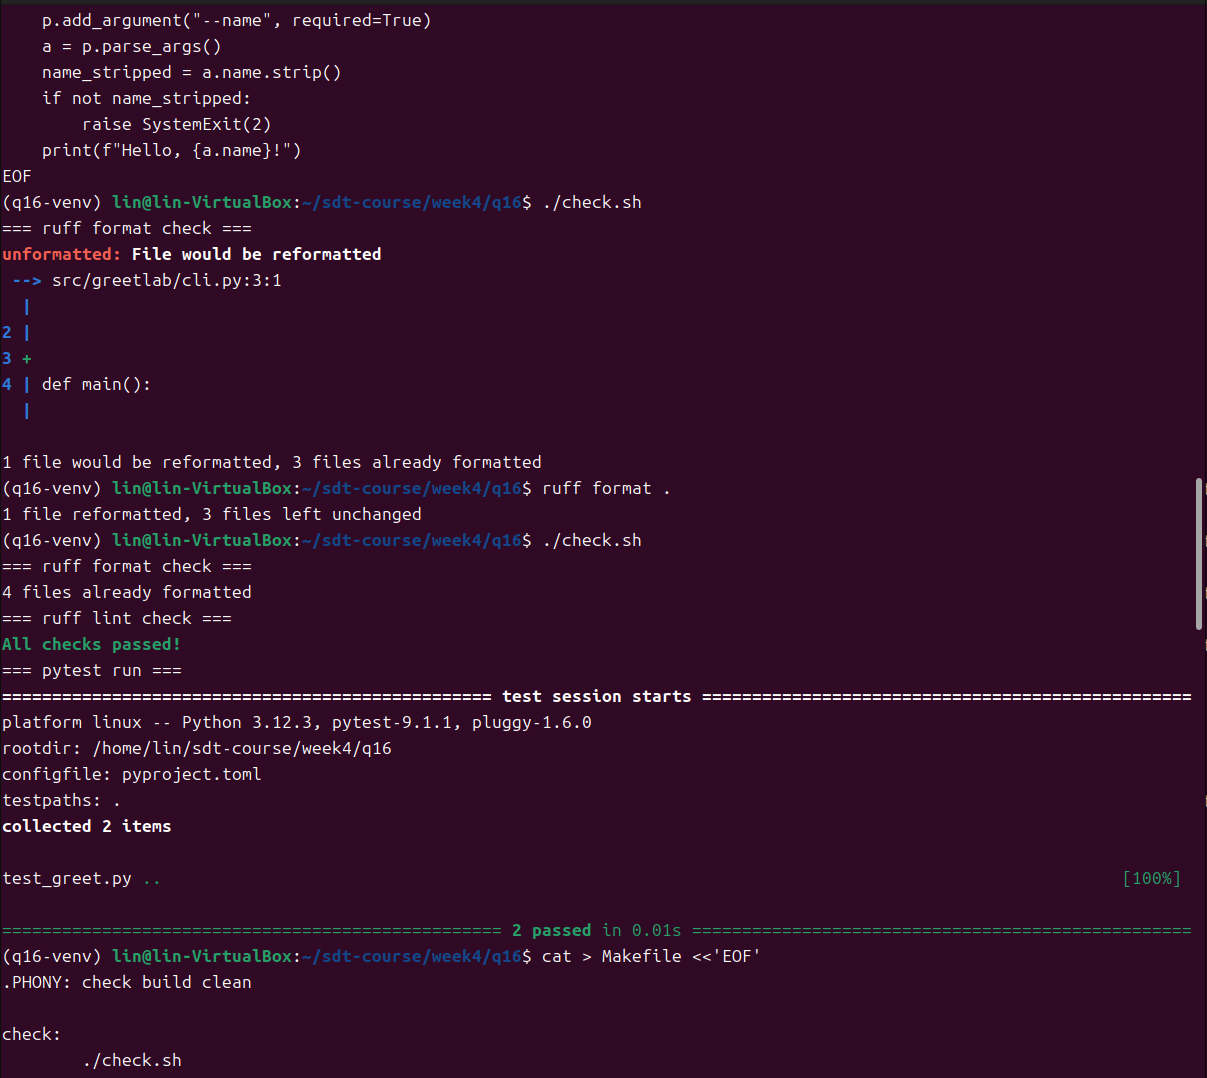
\includegraphics[width=0.9\textwidth]{q16p4.png}
		\caption{q16运行截图24}
		\label{fig:q16_4}
	\end{figure}
	
	\begin{figure}[htbp]
		\centering
		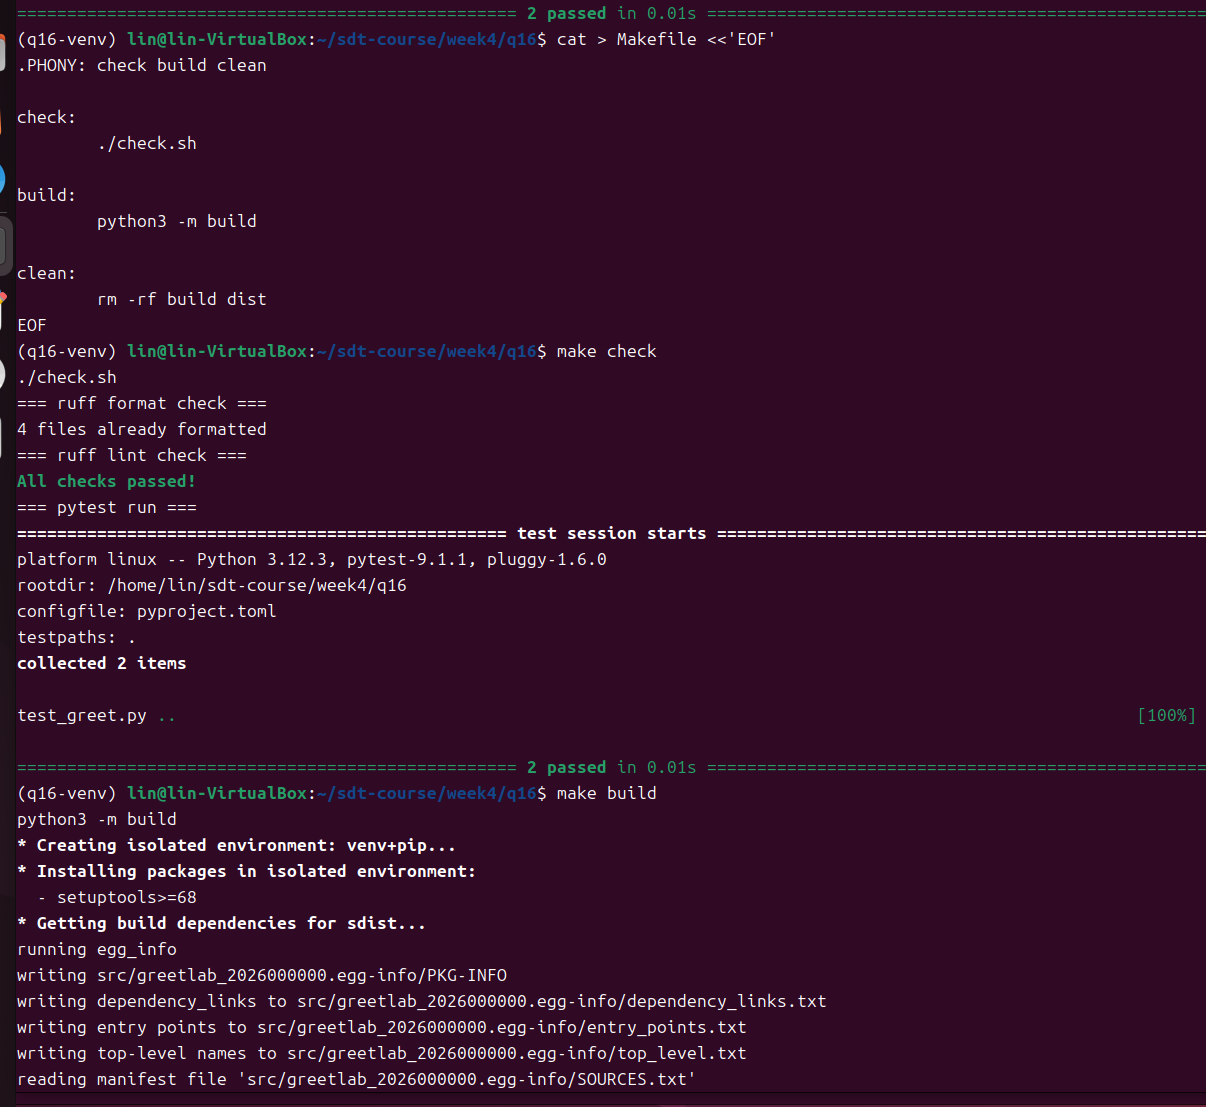
\includegraphics[width=0.9\textwidth]{q16p5.png}
		\caption{q16运行截图5}
		\label{fig:q16_5}
	\end{figure}
	
	\begin{figure}[htbp]
		\centering
		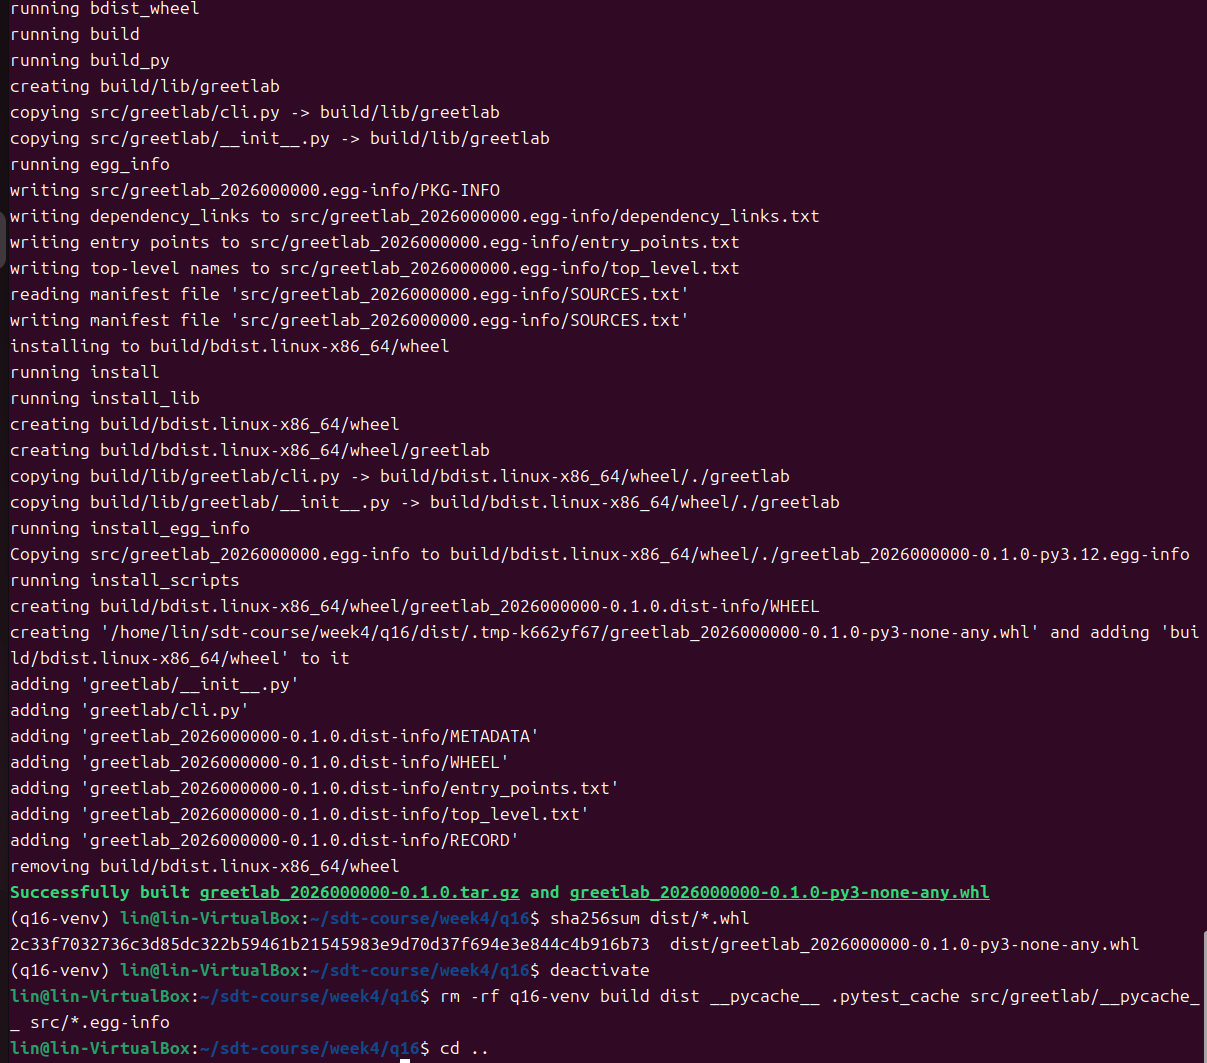
\includegraphics[width=0.9\textwidth]{q16p6.png}
		\caption{q16运行截图6}
		\label{fig:q16_6}
	\end{figure}
	
	\subsubsection{遇到的问题与解决}
	\begin{itemize}
		\item 问题1：Linux系统cp命令不支持\texttt{--exclude}参数，该参数属于rsync工具，直接使用会报参数无法识别。
		
		解决：源目录已经提前清理干净，直接普通\texttt{cp -r}复制；如需过滤文件改用rsync工具。
		
		\item 问题2：重写cli.py制造业务bug时，cat输出引入多余空行，ruff format --check格式校验直接失败，脚本提前终止，pytest没有运行，看不到业务逻辑带来的测试失败。
		
		解决：执行\texttt{ruff format .}修复文件格式，保证格式门禁通过，让pytest可以执行，观察逻辑缺陷造成的测试断言失败。
		
		\item 问题3：Makefile伪目标check/build/clean未加入.PHONY声明；build目标没有调用python3 -m build生成wheel包。
		
		解决：添加\texttt{.PHONY: check build clean}；build配方调用build模块生成wheel，clean删除build、dist打包产物。
		
		\item 问题4：生成wheel后没有计算SHA‑256哈希，缺少题目要求的完整性校验信息。
		
		解决：使用\texttt{sha256sum dist/*.whl}获取wheel文件的sha256摘要。
	\end{itemize}
	
	\section{课后练习}
	
	实例1：虚拟环境环境变量对比
	题目：使用\texttt{printenv}将当前环境变量保存到\texttt{before.txt}；创建Python虚拟环境并激活，再执行\texttt{printenv}保存到\texttt{after.txt}；使用\texttt{diff before.txt after.txt}对比两份文件。观察环境发生了哪些变化？为什么Shell会优先使用虚拟环境内的程序？（提示：重点对比激活前后的\texttt{\$PATH}变量）。执行\texttt{which deactivate}，分析\texttt{deactivate}这个bash函数的工作原理。
	命令：
	\begin{lstlisting}[language=bash]
		printenv > before.txt
		python3 -m venv myvenv
		source myvenv/bin/activate
		printenv > after.txt
		diff before.txt after.txt
		which deactivate
	\end{lstlisting}
	输出：得到两份环境变量文件，diff输出差异，观察\texttt{PATH}变量头部新增虚拟环境bin目录；\texttt{which deactivate}无普通可执行文件输出，确认deactivate为shell内置函数，并非磁盘上独立程序。
	
	实例2：grep正则查找代码中\texttt{subprocess.Popen(..., shell=True)}
	题目：编写正则表达式，使用grep命令行工具，在Python代码文件中查找\texttt{subprocess.Popen}调用且参数包含\texttt{shell=True}的代码行。
	命令：
	\begin{lstlisting}[language=bash]
		grep -nE 'subprocess\.Popen\(.*shell=True\)' *.py
	\end{lstlisting}
	输出：匹配到对应代码行并显示行号；若无匹配内容则无输出。示例命中输出：\texttt{7:    proc = subprocess.Popen(["ls -l /tmp"], shell=True)}。
	
	实例3：正则从JSON字符串捕获name字段值
	题目：给定JSON字符串形如\verb|{"name": "Alyssa P. Hacker", "college": "MIT"}|，编写正则表达式捕获\texttt{name}对应的字段值。
	命令：
	\begin{lstlisting}[language=bash]
		echo '{"name": "Alyssa P. Hacker", "college": "MIT"}' | grep -oP '"name": "\K[^"]+'
	\end{lstlisting}
	输出：
	\begin{lstlisting}
		Alyssa P. Hacker
	\end{lstlisting}
	
	实例4：jq过滤JSON数组，筛选数值大于阈值的元素
	题目：给定JSON数组，筛选\texttt{downloads > 200}的对象，仅输出对象的\texttt{name}字段。
	命令：
	\begin{lstlisting}[language=bash]
		echo '[{"name":"alpha","downloads":120},{"name":"beta","downloads":900},{"name":"gamma","downloads":450}]' | jq -r 'map(select(.downloads>200))[].name'
	\end{lstlisting}
	输出：
	\begin{lstlisting}
		beta
		gamma
	\end{lstlisting}
	
	实例5：find+xargs递归统计项目下py文件总代码行数
	题目：递归查找当前目录全部\texttt{.py}文件，统计全部Python文件的总行数；使用print0与xargs-0兼容文件名含空格场景。
	命令：
	\begin{lstlisting}[language=bash]
		find . -name "*.py" -type f -print0 | xargs -0 cat | wc -l
	\end{lstlisting}
	输出：输出一个整数，代表所有py文件合并后的总行数。
	
	实例6：sed正则捕获组，注释调试print语句
	题目：使用sed捕获组，将形如\texttt{print("debug: x = 123")}调试打印语句注释。
	命令：
	\begin{lstlisting}[language=bash]
		echo 'print("debug: x = 123")' | sed -E 's/^(print\(.*\))/# \1/'
	\end{lstlisting}
	输出：
	\begin{lstlisting}
		# print("debug: x = 123")
	\end{lstlisting}
	
	实例7：Make伪目标演示，观察.PHONY作用
	题目：创建名为\texttt{clean}普通文件，编写Makefile不添加.PHONY，执行make clean；再增加\texttt{.PHONY: clean}再次执行，对比两次行为差异。
	命令：
	\begin{lstlisting}[language=bash]
		touch clean
		cat > Makefile <<'EOF'
		clean:
		rm -f *.tmp
		EOF
		make clean
		cat > Makefile <<'EOF'
		.PHONY: clean
		clean:
		rm -f *.tmp
		EOF
		make clean
	\end{lstlisting}
	输出：无PHONY时提示\verb|make: Nothing to be done for 'clean'|；添加PHONY后会执行rm配方。
	
	实例8：git log正则筛选feat类型提交记录
	题目：筛选git提交历史中提交信息以\texttt{feat:}开头的记录，简短输出哈希与提交说明。
	命令：
	\begin{lstlisting}[language=bash]
		git log --grep='^feat:' --oneline
	\end{lstlisting}
	输出：打印匹配的commit短哈希与提交说明，例如：
	\begin{lstlisting}
		a32bc1f feat: 完成第四周q13 建立可执行的本地质量门禁实验
		67ad211 feat: 完成第四周q14 Make构建系统实验
	\end{lstlisting}
	
	实例9：ruff命令行检测未使用导入
	题目：使用ruff代码质量工具，检测Python源码中未使用的import（F401规则）。
	命令：
	\begin{lstlisting}[language=bash]
		ruff check --select F401 src/
	\end{lstlisting}
	输出：命中未使用导入时输出文件路径、行号与F401告警；无问题则无告警输出。示例：\texttt{src/greetlab/cli.py:2:1: F401 `sys' imported but unused}。
	
	实例10：管道统计模拟日志出现频率最高的ERROR关键词
	题目：给定模拟日志文本，提取ERROR后的关键词，统计出现频次，输出出现次数最高的5个关键词。
	命令：
	\begin{lstlisting}[language=bash]
		cat <<'EOF' | grep -oP 'ERROR: \K\w+' | sort | uniq -c | sort -nr | head -n5
		ERROR: network
		ERROR: disk
		ERROR: network
		ERROR: auth
		ERROR: network
		ERROR: disk
		EOF
	\end{lstlisting}
	输出：
	\begin{lstlisting}
		3 network
		2 disk
		1 auth
	\end{lstlisting}
	
	实例11：jq对JSON数组字段求和
	题目：模拟接口返回JSON数组，计算数组内所有\texttt{downloads}字段数值总和。
	命令：
	\begin{lstlisting}[language=bash]
		echo '[{"name":"a","downloads":10},{"name":"b","downloads":20},{"name":"c","downloads":30}]' | jq '[.[].downloads] | add'
	\end{lstlisting}
	输出：
	\begin{lstlisting}
		60
	\end{lstlisting}
	
	\section{解题感悟}
	第四周实验学习了代码质量门禁、Make构建系统、命令行JSON处理、综合交付测试。本地质量门禁可以将格式化、静态检查、单元测试整合到一条脚本，在提交代码前快速发现问题，提前规避低级错误。Make工具依靠文件时间戳判断是否重新构建，需要准确维护依赖关系，伪目标.PHONY是容易踩坑的关键点。curl+jq可以直接在shell完成JSON数据过滤、排序、报告生成，不需要编写Python脚本。综合交付测试需要完成缺陷复现、定位修复、打包、完整性哈希校验的完整流程。本次实验继续坚持一题一commit，git历史清晰，方便回溯每一步改动。shell正则、管道工具在处理文本、日志、JSON数据时非常高效，适合自动化小脚本开发。
	
	\section{代码仓库提交记录}
	GitHub仓库链接：\url{https://github.com/imnotab/sdtb/tree/main}
	
	\begin{figure}[htbp]
		\centering
		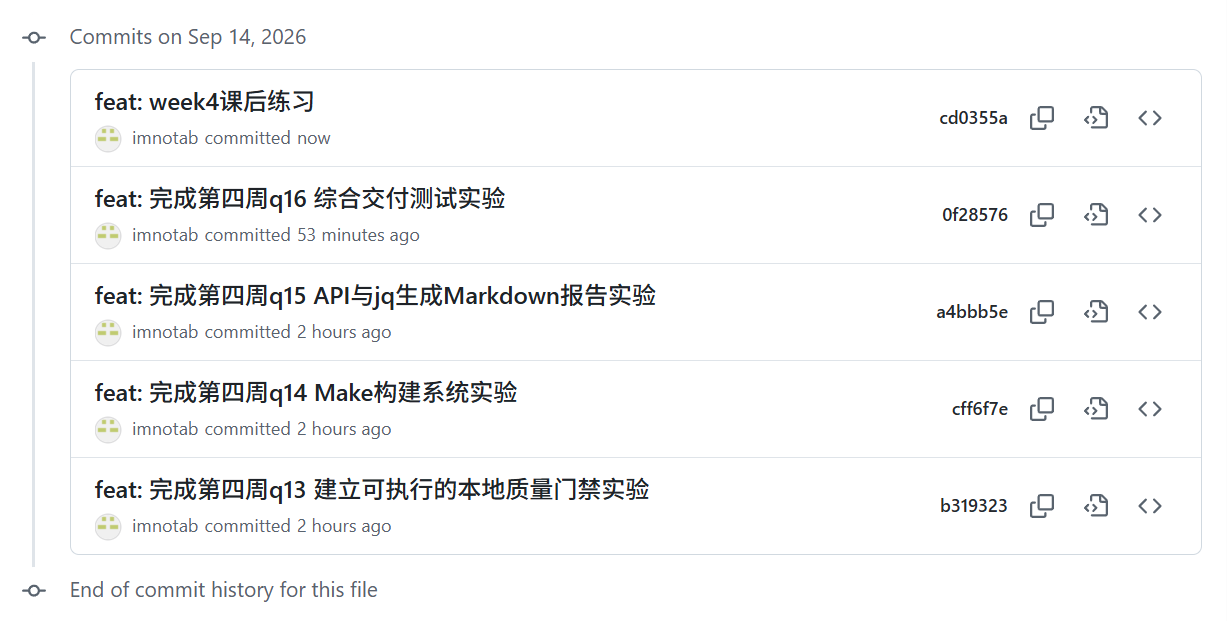
\includegraphics[width=0.9\textwidth]{week4commit.png}
		\caption{项目commit历史记录}
		\label{fig:week4_git}
	\end{figure}
	
\end{document}
